%% Artemis II seismo-acoustic paper -- Seismica submission format
%% Authors: Glenn Thompson (USF), Paul Bremner (NASA MSFC), Han Byul Woo (NASA MSFC), Sue Bilek (NMT) + others
%%
%% Compile from this directory:  ./compile2.sh Artemis2paper.tex
%% Needs seismica.cls, abbrvnat_seismica_upcasetitle.bst and banner.png here.
%%
%% Numbers in this draft come from the notebooks in this folder (run 2026-11-21):
%%   20 clipping, 30 enclosure, 40 moving source + amplitude field, 42 spectral
%%   ratios, 45 sampling rate/bandwidth, 50 coupling, 55 crackle, 60 arrays.

\documentclass[]{seismica}

%% ---- Extra packages ----
\usepackage{amssymb}
\usepackage{booktabs}        % professional tables
\usepackage{longtable}       % multi-page tables
\usepackage{array}
\usepackage{subcaption}

%% ---- Custom commands ----
\newcommand{\todo}[1]{\textcolor{red}{\textbf{[TODO: #1]}}}
\newcommand{\placeholder}[1]{\textcolor{orange}{\textbf{[#1]}}}
\newcommand{\suppfig}[1]{Figure~S#1}
\newcommand{\supptab}[1]{Table~S#1}
\newcommand{\paperone}{Paper~1}
\newcommand{\papertwo}{Paper~2}

%% ---- Figure path ----
\graphicspath{{figures/}}

%% ---- Title and authors ----
\title{The acoustic source of the Artemis~II launch: directivity, crackle and acoustic tracking from a dense seismo-acoustic network}
\shorttitle{The acoustic source of the Artemis~II launch}

%% TODO: + other authors? Authors or acknowledgements?: Jake Anderson,
%% Pati, Dallin, Erin. Acknowledgements: EPIC, Katherine, Don?, Robert,
%% John?, others?
\author[1]{Glenn Thompson\thanks{Corresponding author: \texttt{thompsong@usf.edu}; ORCID: 0000-0002-9173-0097}}
\author[2]{Paul Bremner}
\author[2]{Han Byul Woo}
\author[3]{Sue Bilek}
\affil[1]{University of South Florida, Tampa, Florida, USA}
\affil[2]{NASA Marshall Space Flight Center, Huntsville, Alabama, USA}
\affil[3]{New Mexico Institute of Mining and Technology, Socorro, New Mexico, USA}

%% ---- Document ----
\begin{document}

\makeseistitle{
  \begin{summary}{Abstract}
  %% DRAFT
  We use a dense seismo-acoustic network around the Artemis~II launch of
  the Space Launch System (1~April~2026) to study the acoustic source of
  a heavy-lift rocket. Peak pressure decays with distance as $r^{-1.40}$
  and peak ground velocity as $r^{-1.05}$, with uprange stations
  $\sim$1.4 times louder than downrange ones, and peak arrival times give
  an apparent speed of 127~m~s$^{-1}$. Mapping each station's record to
  the time of emission along a modeled trajectory separates source
  strength, distance and directivity: ignition overpressure dominates to
  the north of the pad, most stations record their strongest
  distance-corrected sound from the first 17--30~s of flight, and
  radiation peaks at $\sim$57$^{\circ}$ from the exhaust axis. A
  point-source model using this measured directivity predicts peak
  arrival times to $\sim$7~s, against 25~s for a 30$^{\circ}$ cone.
  Crackle, measured by the skewness of the pressure derivative, is
  emitted while the vehicle is at 0.2--6~km and subsonic, and increases
  with distance, consistent with shock steepening. Two small arrays of
  low-cost infrasound sensors track the vehicle's bearing from 20 to
  180~s and locate its ground track. High frequencies are lost faster
  along longer paths.
  \end{summary}
  %
  \begin{summary}{Non-technical summary}
  %% DRAFT
  The sound of a rocket launch comes from the rocket's exhaust, which
  moves rapidly upward and away, so the sound heard at any place was
  produced at a different point along the flight. Using several dozen
  microphones and seismometers around the launch pad for NASA's first
  crewed Artemis flight, we worked out which part of the flight produced
  the sound heard at each place. This shows in which directions the
  rocket is loudest, when the characteristic ``crackle'' was produced,
  and how the sound weakens with distance. Two small clusters of
  microphones were able to follow the rocket across the sky using sound
  alone.
  \end{summary}
}

%% ============================================================
\section{Introduction}

Seismic and infrasound signals generated by rocket launches have been
documented in a number of studies and provide a useful means of
observing energetic, repeatable anthropogenic sources
\citep[e.g.,][]{Kanamori1991,Hupe2019,Pilger2021,schuster_rocketquake_2025}.
Launches from Kennedy Space Center and Cape Canaveral Space Force
Station, FL are particularly well suited to such observations due to
their high frequency, diversity of launch vehicles, and accessibility
for ground-based instrumentation.

Since 2016, the University of South Florida (USF) has conducted
intermittent seismic and infrasound monitoring of launches from this
region, resulting in a dataset comprising approximately 140 launches
recorded between 2016 and 2022 \todo{CITE: USF 2016--2022 overview
paper (in preparation; Thompson et al.)\ once available; for now
leave as uncited or note ``Thompson et al., in prep''}. Close-range
seismo-acoustic recordings of the 2016 Falcon~9 AMOS-6 failure at the
adjacent SLC-40 \citep{thompson_amos6_2026} provide a detailed prior
example from the same site. These observations span a wide range of vehicle types and
atmospheric conditions, providing a valuable archive of seismo-acoustic
signals from controlled, high-energy sources. However, the majority of
these launches were recorded by only one to four stations at a time,
limiting the ability to resolve spatial variability in amplitude and
waveform characteristics, as well as source directionality and
propagation effects.

In parallel with these observational efforts, launch activity from
Kennedy Space Center and Cape Canaveral Space Force Station has
increased substantially over the past decade. This increase is driven in
part by the expansion of commercial launch providers, as well as
continued governmental investment in space exploration. The resulting
growth in launch cadence and diversity of vehicle classes---including
the introduction of heavy- and super-heavy-lift systems associated with
the Artemis program---provides new opportunities for detailed
seismo-acoustic observation. Rocket launches constitute repeatable,
high-energy, and well-timed sources, with known origin times and
locations, making them well suited for investigating source radiation
characteristics, propagation through the atmosphere and solid Earth, and
coupling between air pressure and ground motion.

The 2026 Artemis~II launch represents a particularly compelling case
study. As the first crewed mission of the Artemis program, it marks a
major milestone in human spaceflight and is powered by the Space Launch
System (SLS), one of the most energetic launch vehicles ever operated
from this region \citep{NASA_SLS,Sutton2017}. A precursor to this effort, the Artemis~I launch in 2022,
was recorded by a limited network of four stations, demonstrating the
detectability and complexity of the signals generated by the SLS but
also highlighting the limitations imposed by sparse spatial sampling.

Rocket noise is generated by the exhaust jet of a vehicle that
accelerates, climbs and turns, so the sound arriving at a station at a
given time was emitted earlier, from a different position, in a
different direction relative to the exhaust. Peak amplitudes and arrival
times at a network therefore mix source strength, distance and
directivity. Here we use the dense network deployed for Artemis~II,
validated in a companion paper (\paperone), to separate them. We
(1)~describe the amplitude field of pressure and ground motion with
distance and azimuth; (2)~map every station's record to the time of
emission along a modeled trajectory; (3)~measure the radiation pattern
and use it in a simple forward model; (4)~track the vehicle with two
small infrasound arrays; and (5)~quantify crackle, the shock-dominated
component of rocket noise, and where along the flight it is produced.

%% ============================================================
\section{Network and Data}
\label{sec:data}

The network, its validation and the processing are described in the
companion paper (\paperone). In brief, during the launch on 1~April~2026 (22:35:12~UTC)
about 40 sensors operated at 0.7--7.6~km from Space Launch Complex 39B
(SLC-39B; Figure~\ref{fig:station_map}; coordinates in \supptab{1}):
Nanometrics Trillium Compact seismometers and infraBSU microbarometers
(housed in the plastic totes that also enclosed the electronics) on 24-bit
Centaur digitizers at 500~samples~s$^{-1}$ (B01, B03, B05, B29),
22 Gem infrasound loggers (16-bit, 100~samples~s$^{-1}$) and 11 SmartSolo
5~Hz nodes. Two clusters of Gems form small arrays: B20 (five Gems within
$\sim$35~m, 7.6~km south-east of the pad) and B24 (four Gems within
$\sim$250~m, 5.5~km south-south-west).

All records were corrected to pressure or ground velocity with the
digitizers' own response files and the sensor responses; SmartSolo data,
recorded as geophone voltage with reversed vertical polarity, were
corrected with the nominal 5~Hz response and used above 1~Hz. Six Gem
channels within 3.4~km overflowed for 14--29~s above
$\sim$100--140~Pa; their overflow intervals are masked throughout, while
the records before and after are used (\paperone). B03's Centaur channels
(hardware fault) and B05's seismometer (off-centre mass) are excluded from
quantitative fits. Because rocket signal lies almost entirely above
0.5~Hz in pressure and 1~Hz in ground motion (\paperone), pressure and
velocity are high-passed at 0.5~Hz and 1~Hz. Peak amplitudes are measured
in the first 180~s after launch over unmasked samples; stations east of
the pad (azimuth 0--180$^{\circ}$; B14, B01, B07, B23, B20) lie downrange
and those to the west (B03, B05, B12, B24, B29) uprange.

\begin{figure}[htbp]
  \centering
  %% Source: Box .../writing/Artemis2/artemis2_infrasound_map_abs_peak.pdf
  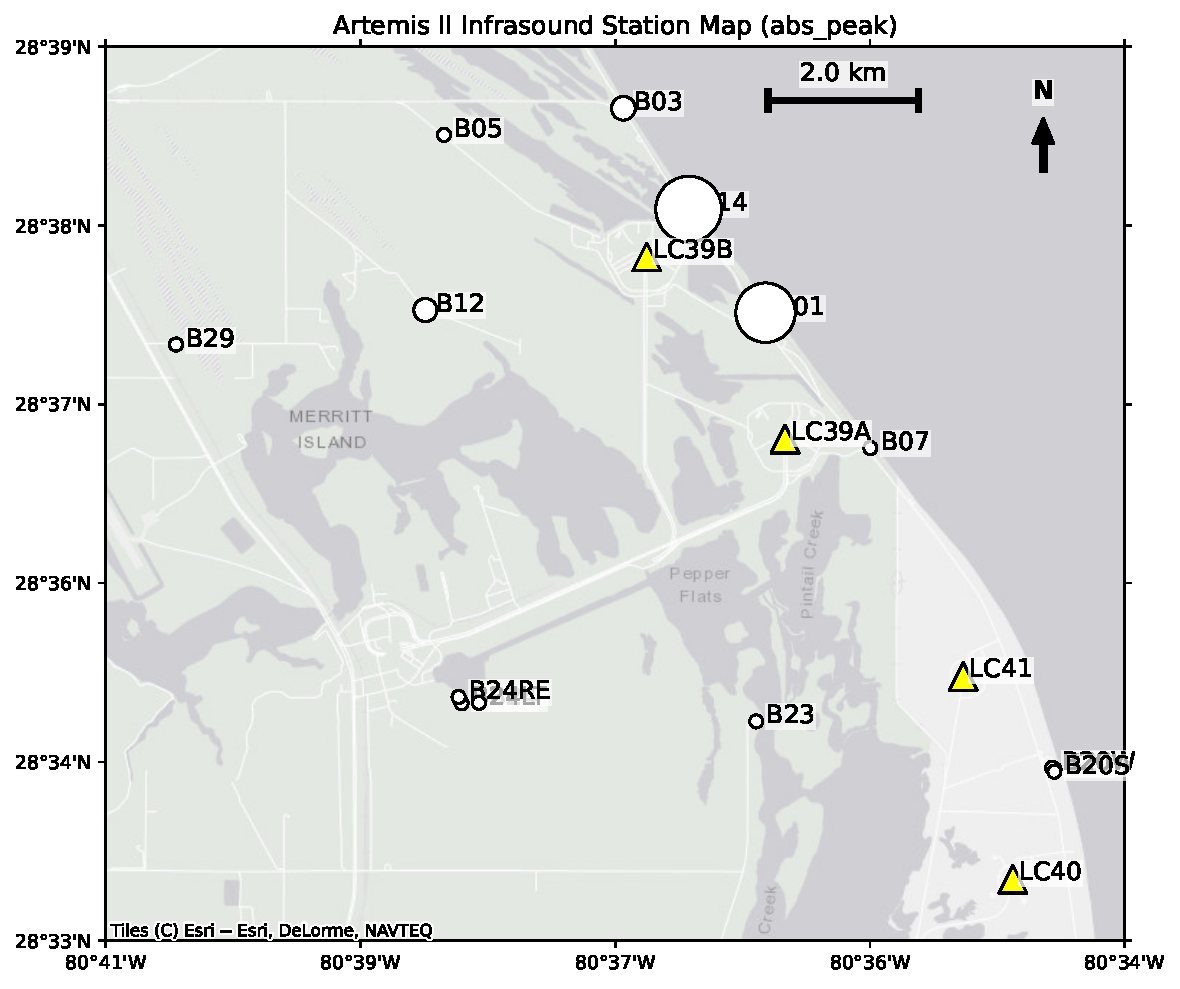
\includegraphics[width=0.95\textwidth]{figures/station_map}
  \caption{Map of infrasound stations (circles) and active launch
    complexes (yellow triangles) for the Artemis~II launch from
    SLC-39B. Station symbols are scaled by peak absolute infrasound
    amplitude. \todo{Regenerate with overflowed Gem channels shown as
    lower bounds (notebook 25).}}
  \label{fig:station_map}
\end{figure}


%% ============================================================
\section{First Look at the Signals}
\label{sec:spectral}

Figure~\ref{fig:nearfar}a compares a near (B01, 1.5~km) and a far
(B29, 5.6~km) station. Both record broadband pressure and ground motion
extending to the top of the 500~samples~s$^{-1}$ band. The near
station's record is dominated by the first $\sim$40~s of flight; the far
station's is lower, later and broader. As the vehicle climbs, high
frequencies decline. The spectral centroid of pressure (4-s windows,
mapped to source time) peaks at $\sim$40--45~Hz at B01 and
$\sim$30~Hz at B29 for sound emitted 12--18~s after liftoff, and falls to
6--9~Hz at B01 but 2--5~Hz at B29 for sound emitted 60--100~s after
liftoff (Figure~\ref{fig:nearfar}b). The stronger loss of high frequencies along the
longer paths to the far station anticipates the steeper-than-$1/r$
decay of peak pressure (Section~\ref{sec:amplitude}). The spectral
centroid is plotted against source time, the time at which the sound left
the vehicle, which is defined in Section~\ref{sec:trajectory}; the
records of every station are shown in \paperone.

\begin{figure}[htbp]
  \centering
  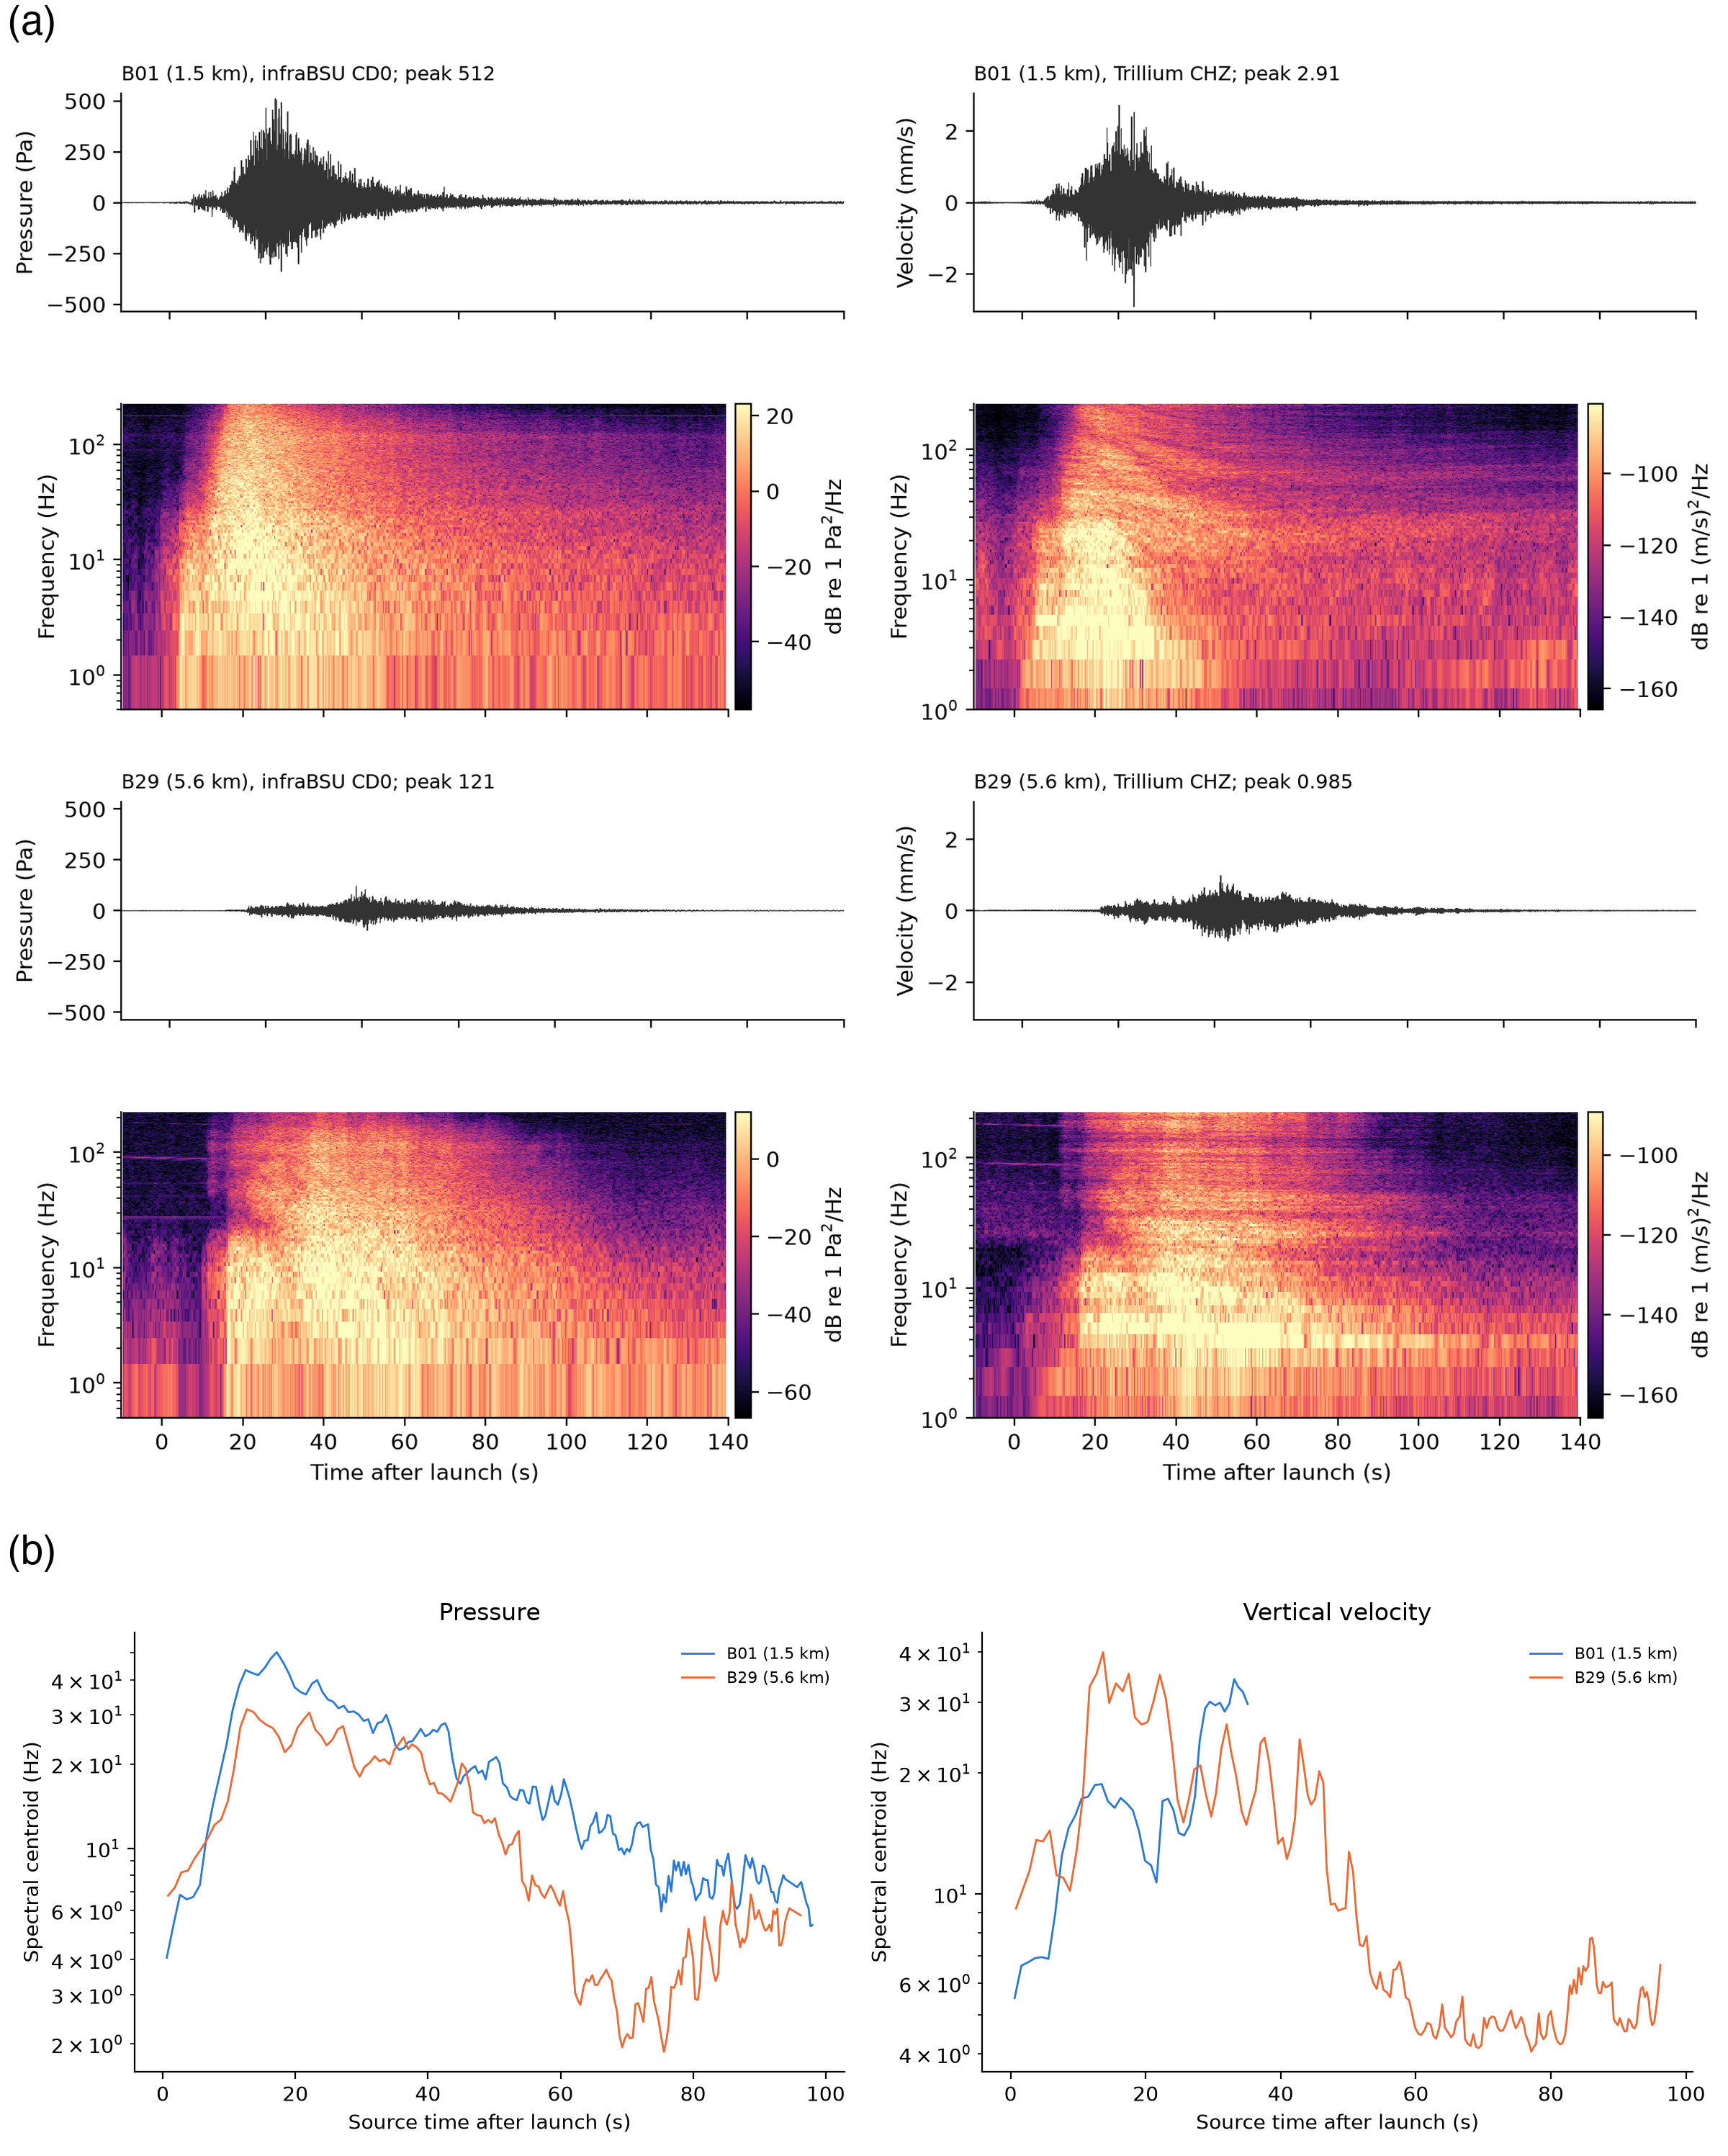
\includegraphics[width=0.85\textwidth]{composite_near_far}
  \caption{(a) Pressure (infraBSU DD0, $>$0.5~Hz; left) and vertical ground
    velocity (Trillium DHZ, $>$1~Hz; right) at B01 (1.5~km from SLC-39B)
    and B29 (5.6~km), each with its spectrogram (512-sample windows).
    (b) Spectral centroid of pressure and vertical velocity in 4-s windows,
    plotted at the source time of emission (Section~\ref{sec:trajectory});
    windows less than ten times the pre-launch noise are omitted.}
  \label{fig:nearfar}
\end{figure}


%% ============================================================
\section{Trajectory Model and Source-Time Mapping}
\label{sec:trajectory}

To relate each station's record to the part of the flight that produced
it, we use an idealized model of the trajectory: the vehicle ascends
vertically and then pitches over downrange in a gravity turn. Sound is
assumed to travel along straight rays at a constant 343~m~s$^{-1}$,
neglecting stratification and wind, which is reasonable while the
vehicle is below $\sim$10~km (the first $\sim$60~s) and increasingly
approximate afterwards. The trajectory is 2-D (downrange distance and
altitude); we place it on the map along a launch azimuth of
90$^{\circ}$, which the infrasound arrays support
(Section~\ref{sec:arrays}).

\subsection{Trajectory}

Model parameters were selected to approximate the early flight profile
of the Artemis~II launch. The nominal thrust is 37.4~MN (corresponding
to 8.4~million~lbf average over the first two minutes), with a simple
throttle schedule applied: full thrust for the first 60~s, reduced to
88\% between 60--80~s, then 95\% between 80--128~s. The initial vehicle
mass is $2.61\times10^{6}$~kg, with a constant mass depletion rate of
\SI{12081}{\kilo\gram\per\second}, representing propellant consumption
by the core stage and solid rocket boosters. Gravitational acceleration
is fixed at \SI{9.81}{\metre\per\second\squared}.

The pitch program is defined by three parameters: an initial vertical
ascent of 6~s, a brief 2$^{\circ}$ pitchover beginning at 10~s, and a
constant pitch rate of 0.45$^{\circ}$~s$^{-1}$ thereafter up to a
maximum pitch angle of 80$^{\circ}$.

Aerodynamic drag is included using a Mach-dependent drag coefficient
(subsonic $C_D \approx 0.30$, rising to 0.60 at transonic, declining to
0.35 at supersonic), with a reference area of 78~m$^2$ and an
exponentially decreasing atmospheric density profile (sea-level density
1.225~kg~m$^{-3}$, scale height 8.5~km). The local sound speed for
Mach number calculation uses a tropospheric temperature lapse rate of
6.5~K~km$^{-1}$, constant below 11~km.

The modeled vehicle reaches 1~km altitude at 20~s, 2.3~km at 30~s,
10~km at 60~s and 45~km at 120~s, passing Mach~1 at $\sim$48~s
(Figure~\ref{fig:trajectory}; velocity components in \suppfig{5}).

\begin{figure}[htbp]
  \centering
  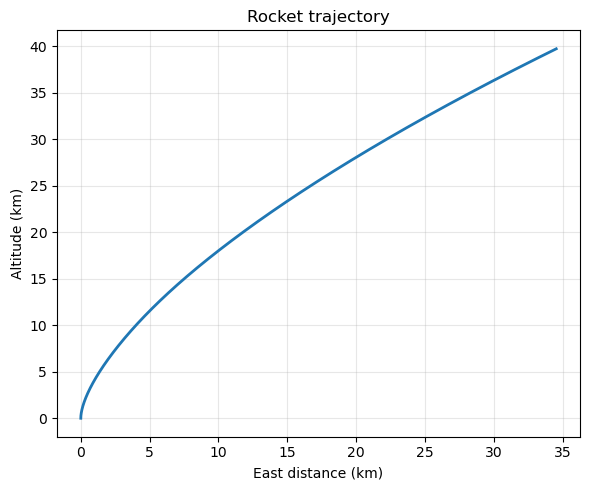
\includegraphics[width=0.8\textwidth]{figures/trajectory}
  \caption{Modeled rocket trajectory during the first 120~s of flight,
    showing altitude as a function of downrange distance.}
  \label{fig:trajectory}
\end{figure}

\subsection{Source-Time Mapping}

For each station and each source time $t_s$, the model gives the
source--receiver distance $R(t_s)$, the arrival time
$t_\text{obs} = t_s + R(t_s)/c$, the emission angle $\phi$ between the
exhaust direction (anti-parallel to the velocity) and the ray to the
station, and the ray's elevation angle. Within the first 150~s,
$dt_\text{obs}/dt_s$ remains positive at every station, so each arrival
time corresponds to a single source time, and any measurement made on a
record can be assigned to the time, altitude and emission angle at which
the sound left the vehicle.


%% ============================================================
\section{Amplitude Field and Arrival Times}
\label{sec:amplitude}

\subsection{Peak Pressure and Ground Velocity versus Distance}
\label{sec:pgv}

Excluding overflowed Gems (whose unclipped peaks are lower bounds) and
faulty channels, peak pressure decays as
\begin{equation}
  p_\text{pk} = 927\,r^{-1.40}~\text{Pa}
  \label{eq:amplitude_decay}
\end{equation}
and peak vertical ground velocity as
\begin{equation}
  v_\text{pk} = 4.9\times10^{-3}\,r^{-1.05}~\text{m~s}^{-1}
  \label{eq:pgv_decay}
\end{equation}
with $r$ in km (Figure~\ref{fig:amplitude}, \supptab{2});
the scatter about both fits is 0.09 log units (17 pressure and 12
velocity channels). The largest recorded pressure was 512~Pa
(148~dB peak) at B01, 1.5~km from the pad; the overflowed Gems at
B14 (0.7~km) would have recorded more. Pressure decays considerably
faster than $1/r$, whereas peak
ground velocity decays close to $1/r$. Part of the pressure decay
reflects source motion: the closest stations peak early, when the
vehicle is near the ground and close to them, whereas the farthest peak
later from a source several kilometres up (Section~\ref{sec:moving}).
Part reflects the loss of high frequencies at 100~samples~s$^{-1}$, since
the farther stations are all Gems. A previous fit to these data
($R^{-1.22}$) included overflowed Gem channels and is superseded.

Residuals about Equation~\ref{eq:amplitude_decay} differ by azimuth:
uprange (west) channels average $+0.08$ log units and downrange (east)
channels $-0.07$, so at a given distance uprange stations are
$\sim$1.4 times louder in peak pressure.

\begin{figure}[htbp]
  \centering
  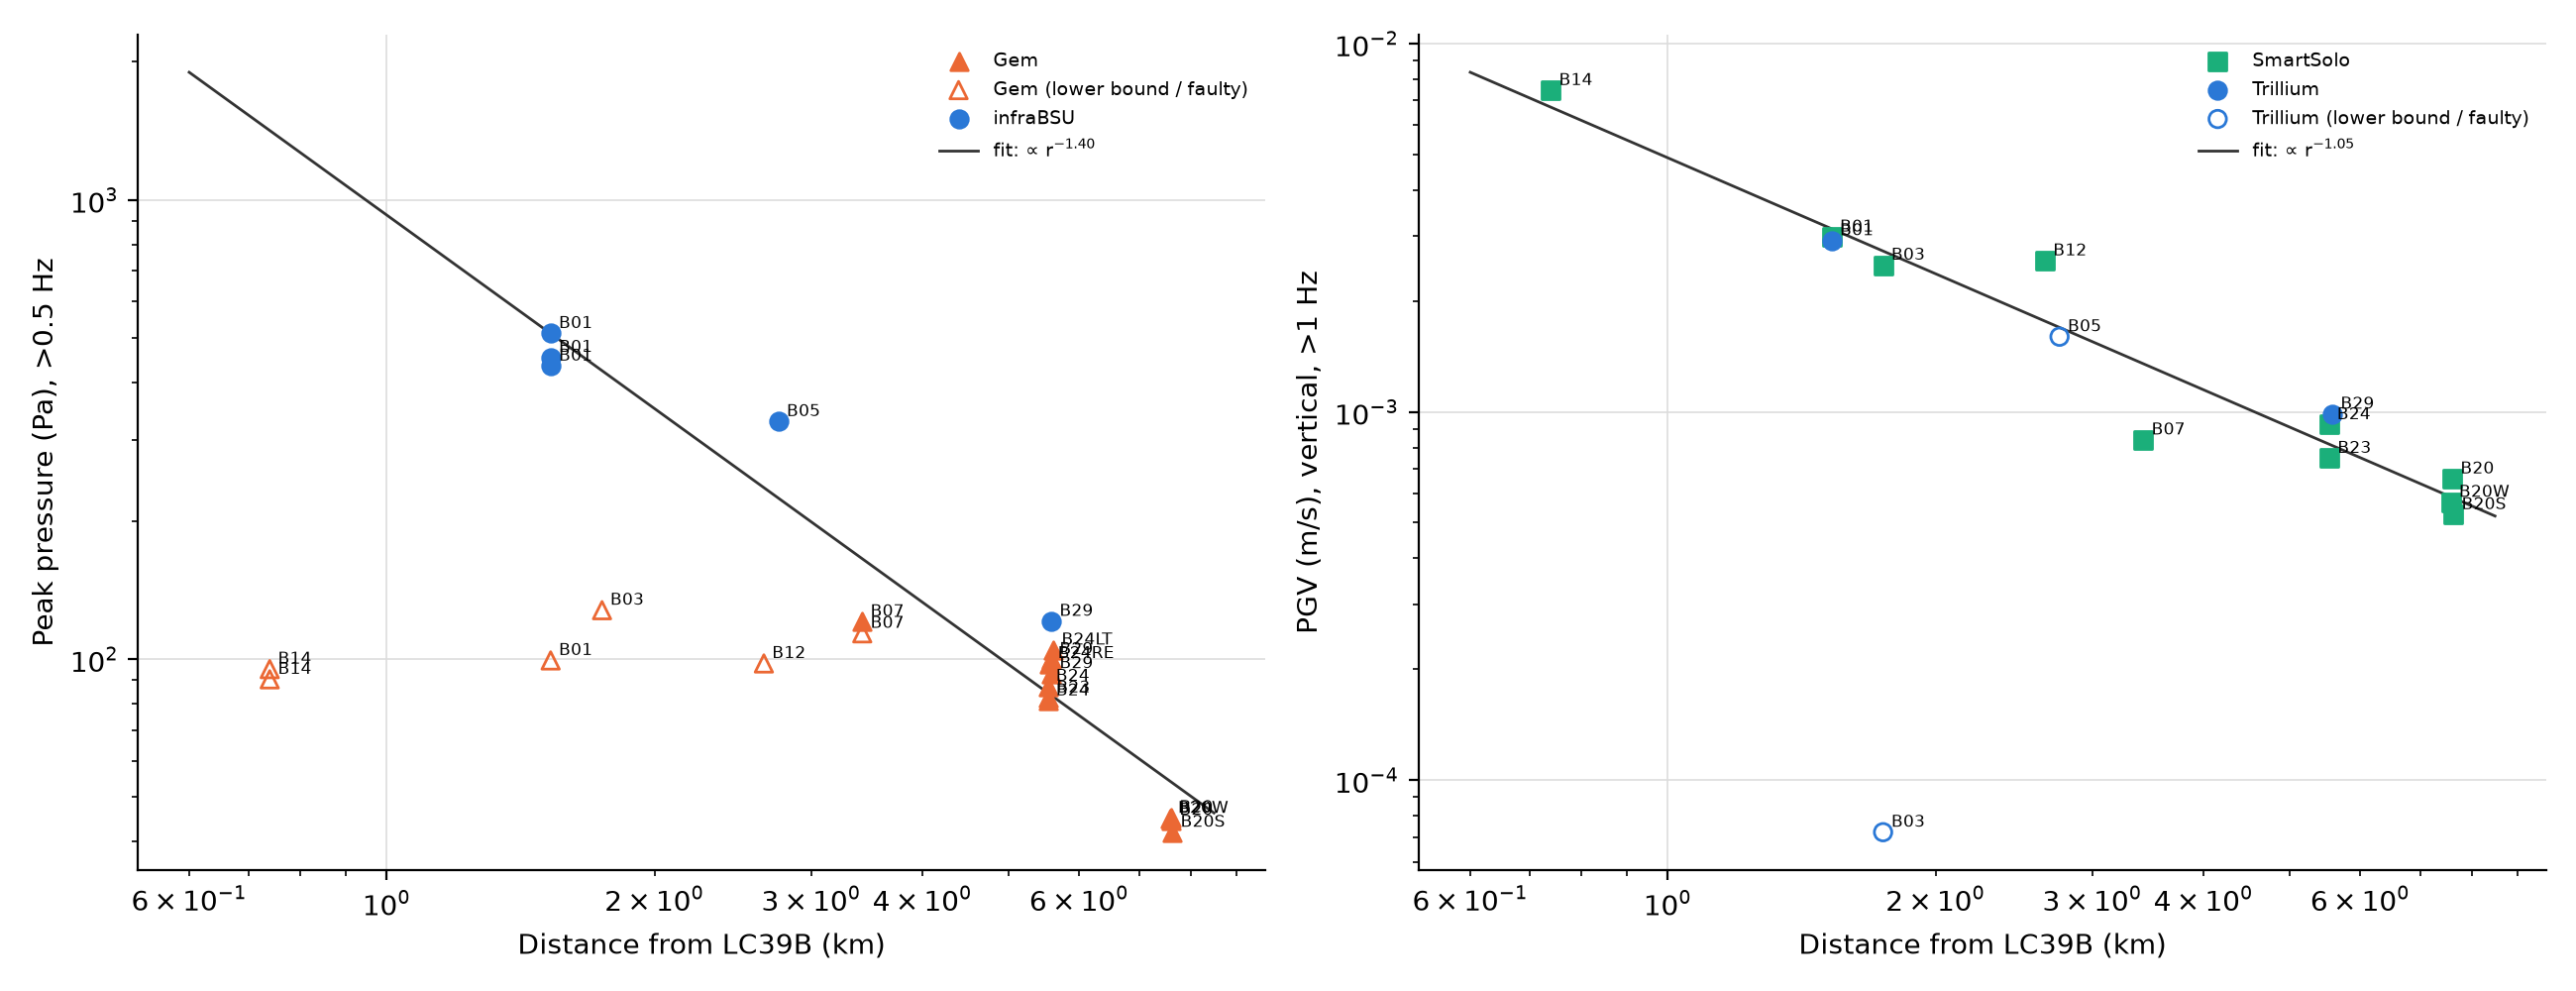
\includegraphics[width=\textwidth]{amplitude_field}
  \caption{Left: peak pressure ($>$0.5~Hz) versus distance; open
    symbols are overflowed Gems, whose unclipped peak is a lower bound.
    Right: peak vertical ground velocity ($>$1~Hz) for Trillium and
    SmartSolo sensors; open symbols are the faulty B03 and drifting B05
    Trillium channels. Lines: power-law fits to the filled symbols.}
  \label{fig:amplitude}
\end{figure}

\subsection{Arrival Times}
\label{sec:arrival_times}

Peak pressure arrival times (\supptab{2}, excluding
overflowed channels) increase with distance as $t = 2.6 + 7.9\,r$~s
($r$ in km), an apparent speed of 127~m~s$^{-1}$, far below the sound
speed. The slowness arises because the loudest sound reaching distant stations was emitted later,
from higher on the trajectory. At similar distances uprange stations
peak earlier than downrange ones (38.7--39.0~s at B24 and B29 versus
45.5~s at B23, all at 5.5~km). The record
section of pressure envelopes (Figure~\ref{fig:record_section}) shows
that the arrival curves predicted for successive source times track the
evolution of the observed envelopes. Peak times are compared with a
source model in Section~\ref{sec:model}.

Signal onsets reveal a second source. Interpreted as straight-ray
arrivals from the pad, the onsets at the nearer and quieter stations
imply emission 3--6~s before liftoff, consistent with the start of the
core-stage engines, whereas the farthest stations (B20, B07, B23) first
detect the louder booster ignition at $\sim$0~s. Onset detection depends
on each sensor's noise level (Gems at the same site differ by up to
4~s), so onsets are used only qualitatively.

\begin{figure}[htbp]
  \centering
  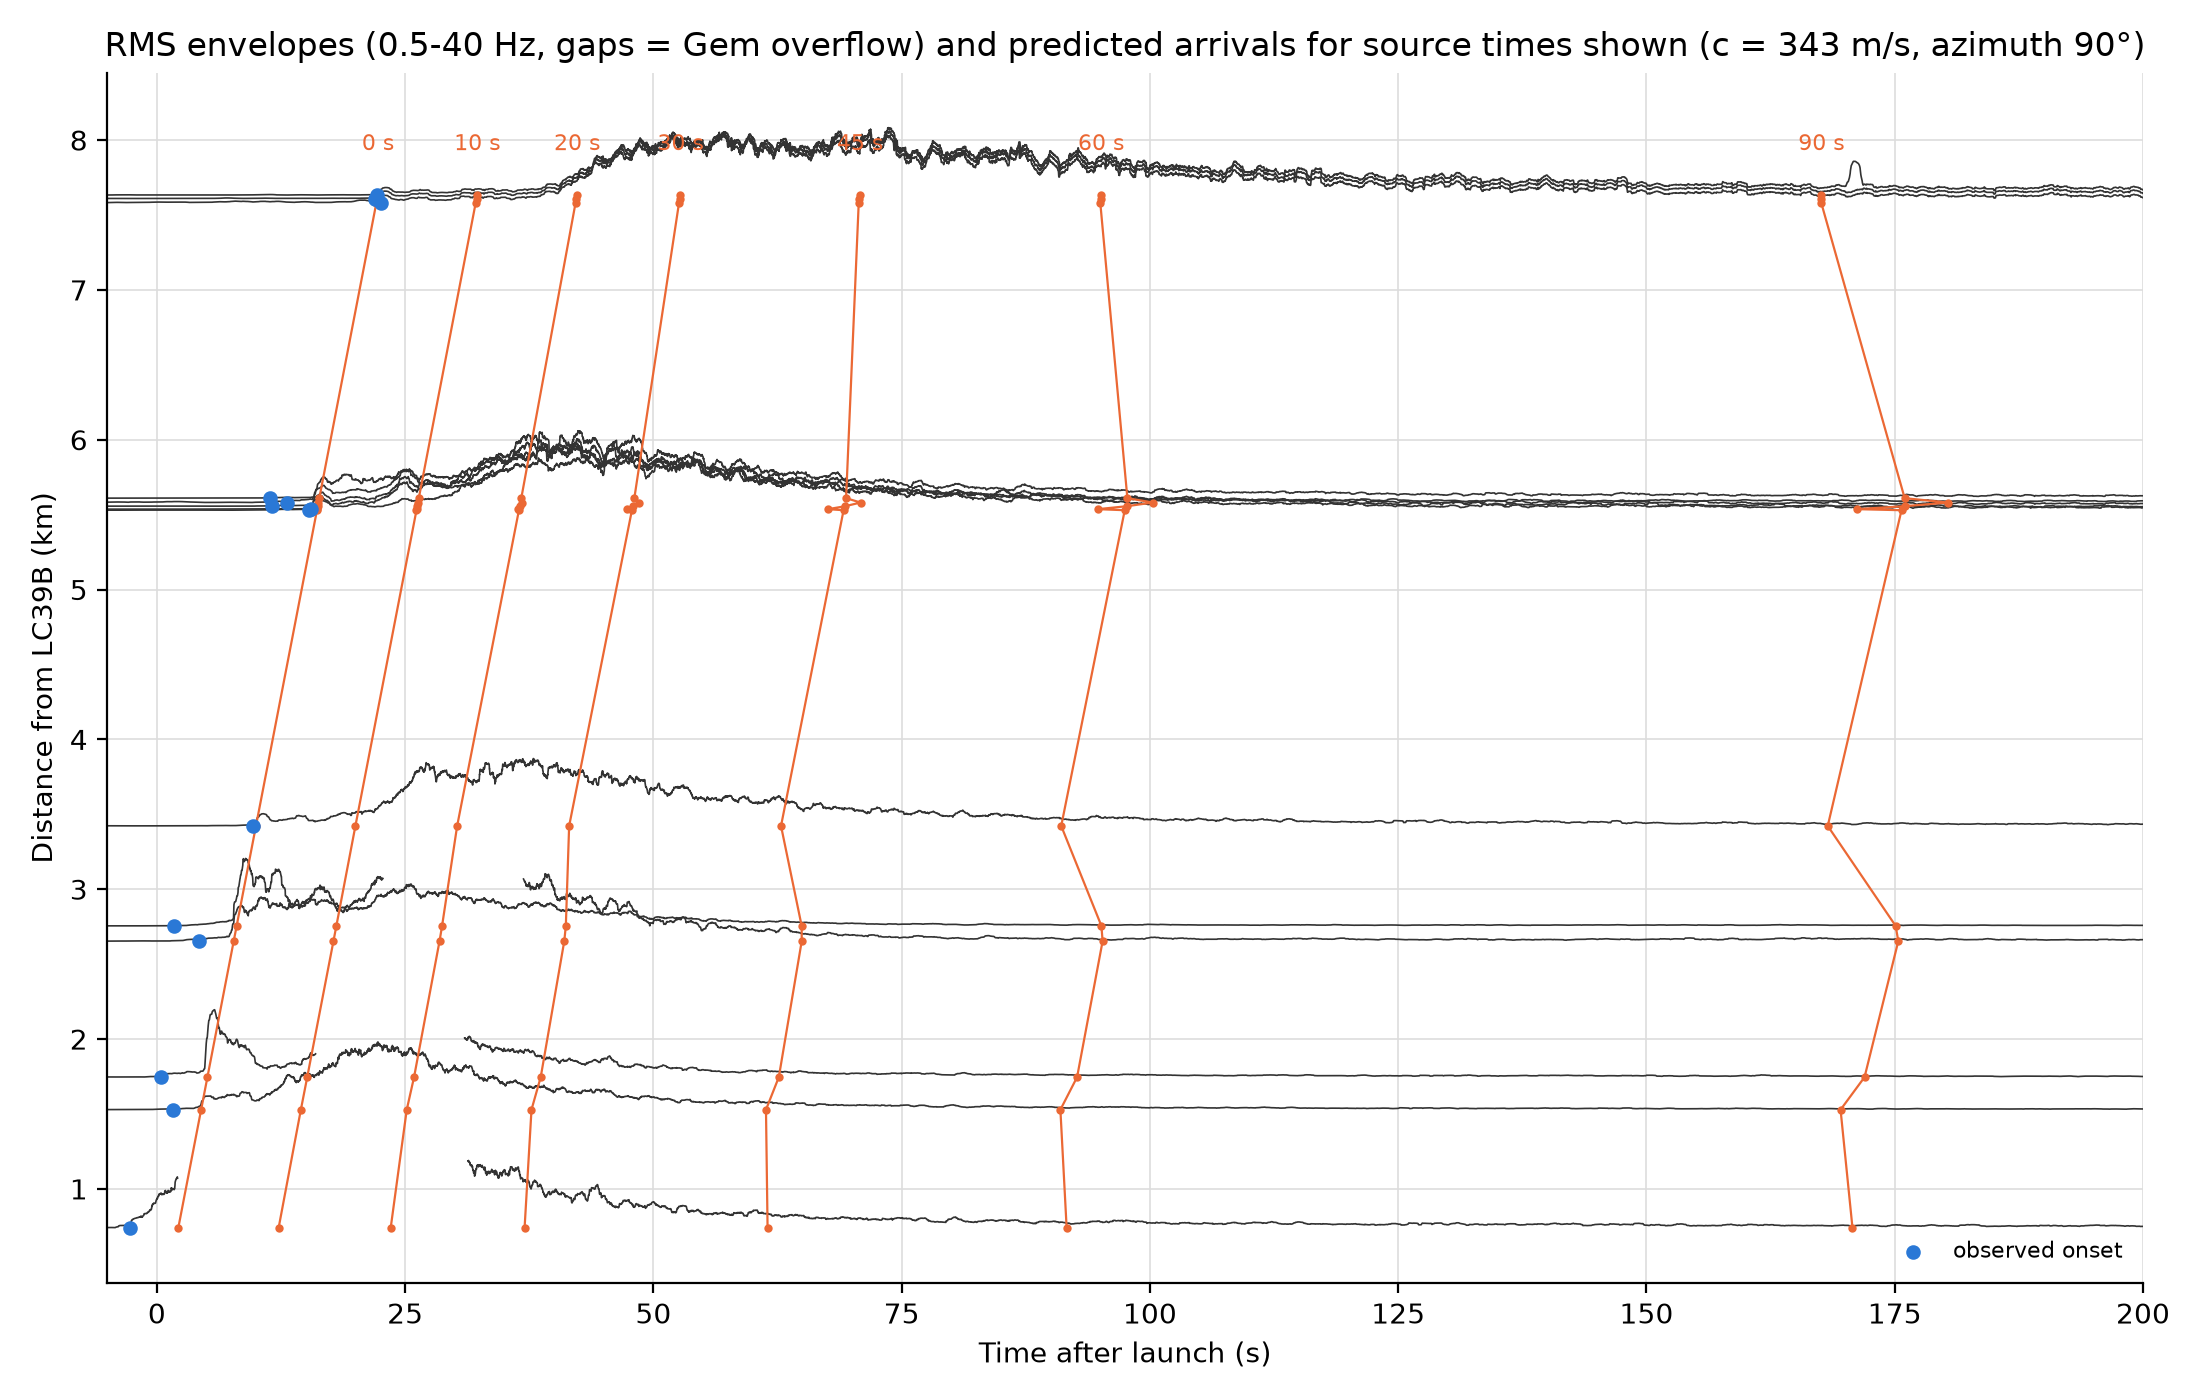
\includegraphics[width=\textwidth]{moving_source_record_section}
  \caption{Pressure envelopes (RMS in 1-s windows, 0.5--40~Hz; gaps are
    Gem overflow intervals) plotted at each station's distance, with
    the arrival times predicted for sound emitted at the source times
    shown (orange; straight rays, $c = 343$~m~s$^{-1}$, launch azimuth
    90$^{\circ}$). Blue dots: detected onsets.}
  \label{fig:record_section}
\end{figure}


%% ============================================================
\section{Moving-Source Analysis}
\label{sec:moving}

\subsection{Amplitude in Source Time}

Each station's pressure envelope was read at the arrival time predicted
for every source time $t_s$ (0.5~s steps), giving an amplitude history in
source time; multiplying by $R(t_s)$ removes spherical spreading
(``reduced pressure'', Pa~km). Overflow intervals and windows with a
signal-to-noise ratio below 3 are omitted, so the near stations
contribute only for source times when they were not saturated, and the
overlap with farther stations ties the network together without a
separate amplitude calibration ladder.

The result (Figure~\ref{fig:reduced}) separates three phases. At
$t_s \lesssim 5$~s, the stations north of the pad (B03 and B05) record
their largest reduced pressures, up to 270~Pa~km, while stations to the
south-east (the B20 cluster) record their weakest; this is ignition
overpressure and pad noise, radiated preferentially northward,
consistent with the orientation of the flame trench. Between
$t_s \approx 17$ and 30~s, with the vehicle at 0.8--2.3~km, nearly every
station reaches its maximum reduced pressure of 130--175~Pa~km. After
$t_s \approx 45$~s the downrange stations remain up to twice as loud as
the uprange stations, until the two groups converge at
$t_s \approx 100$~s.

\begin{figure}[htbp]
  \centering
  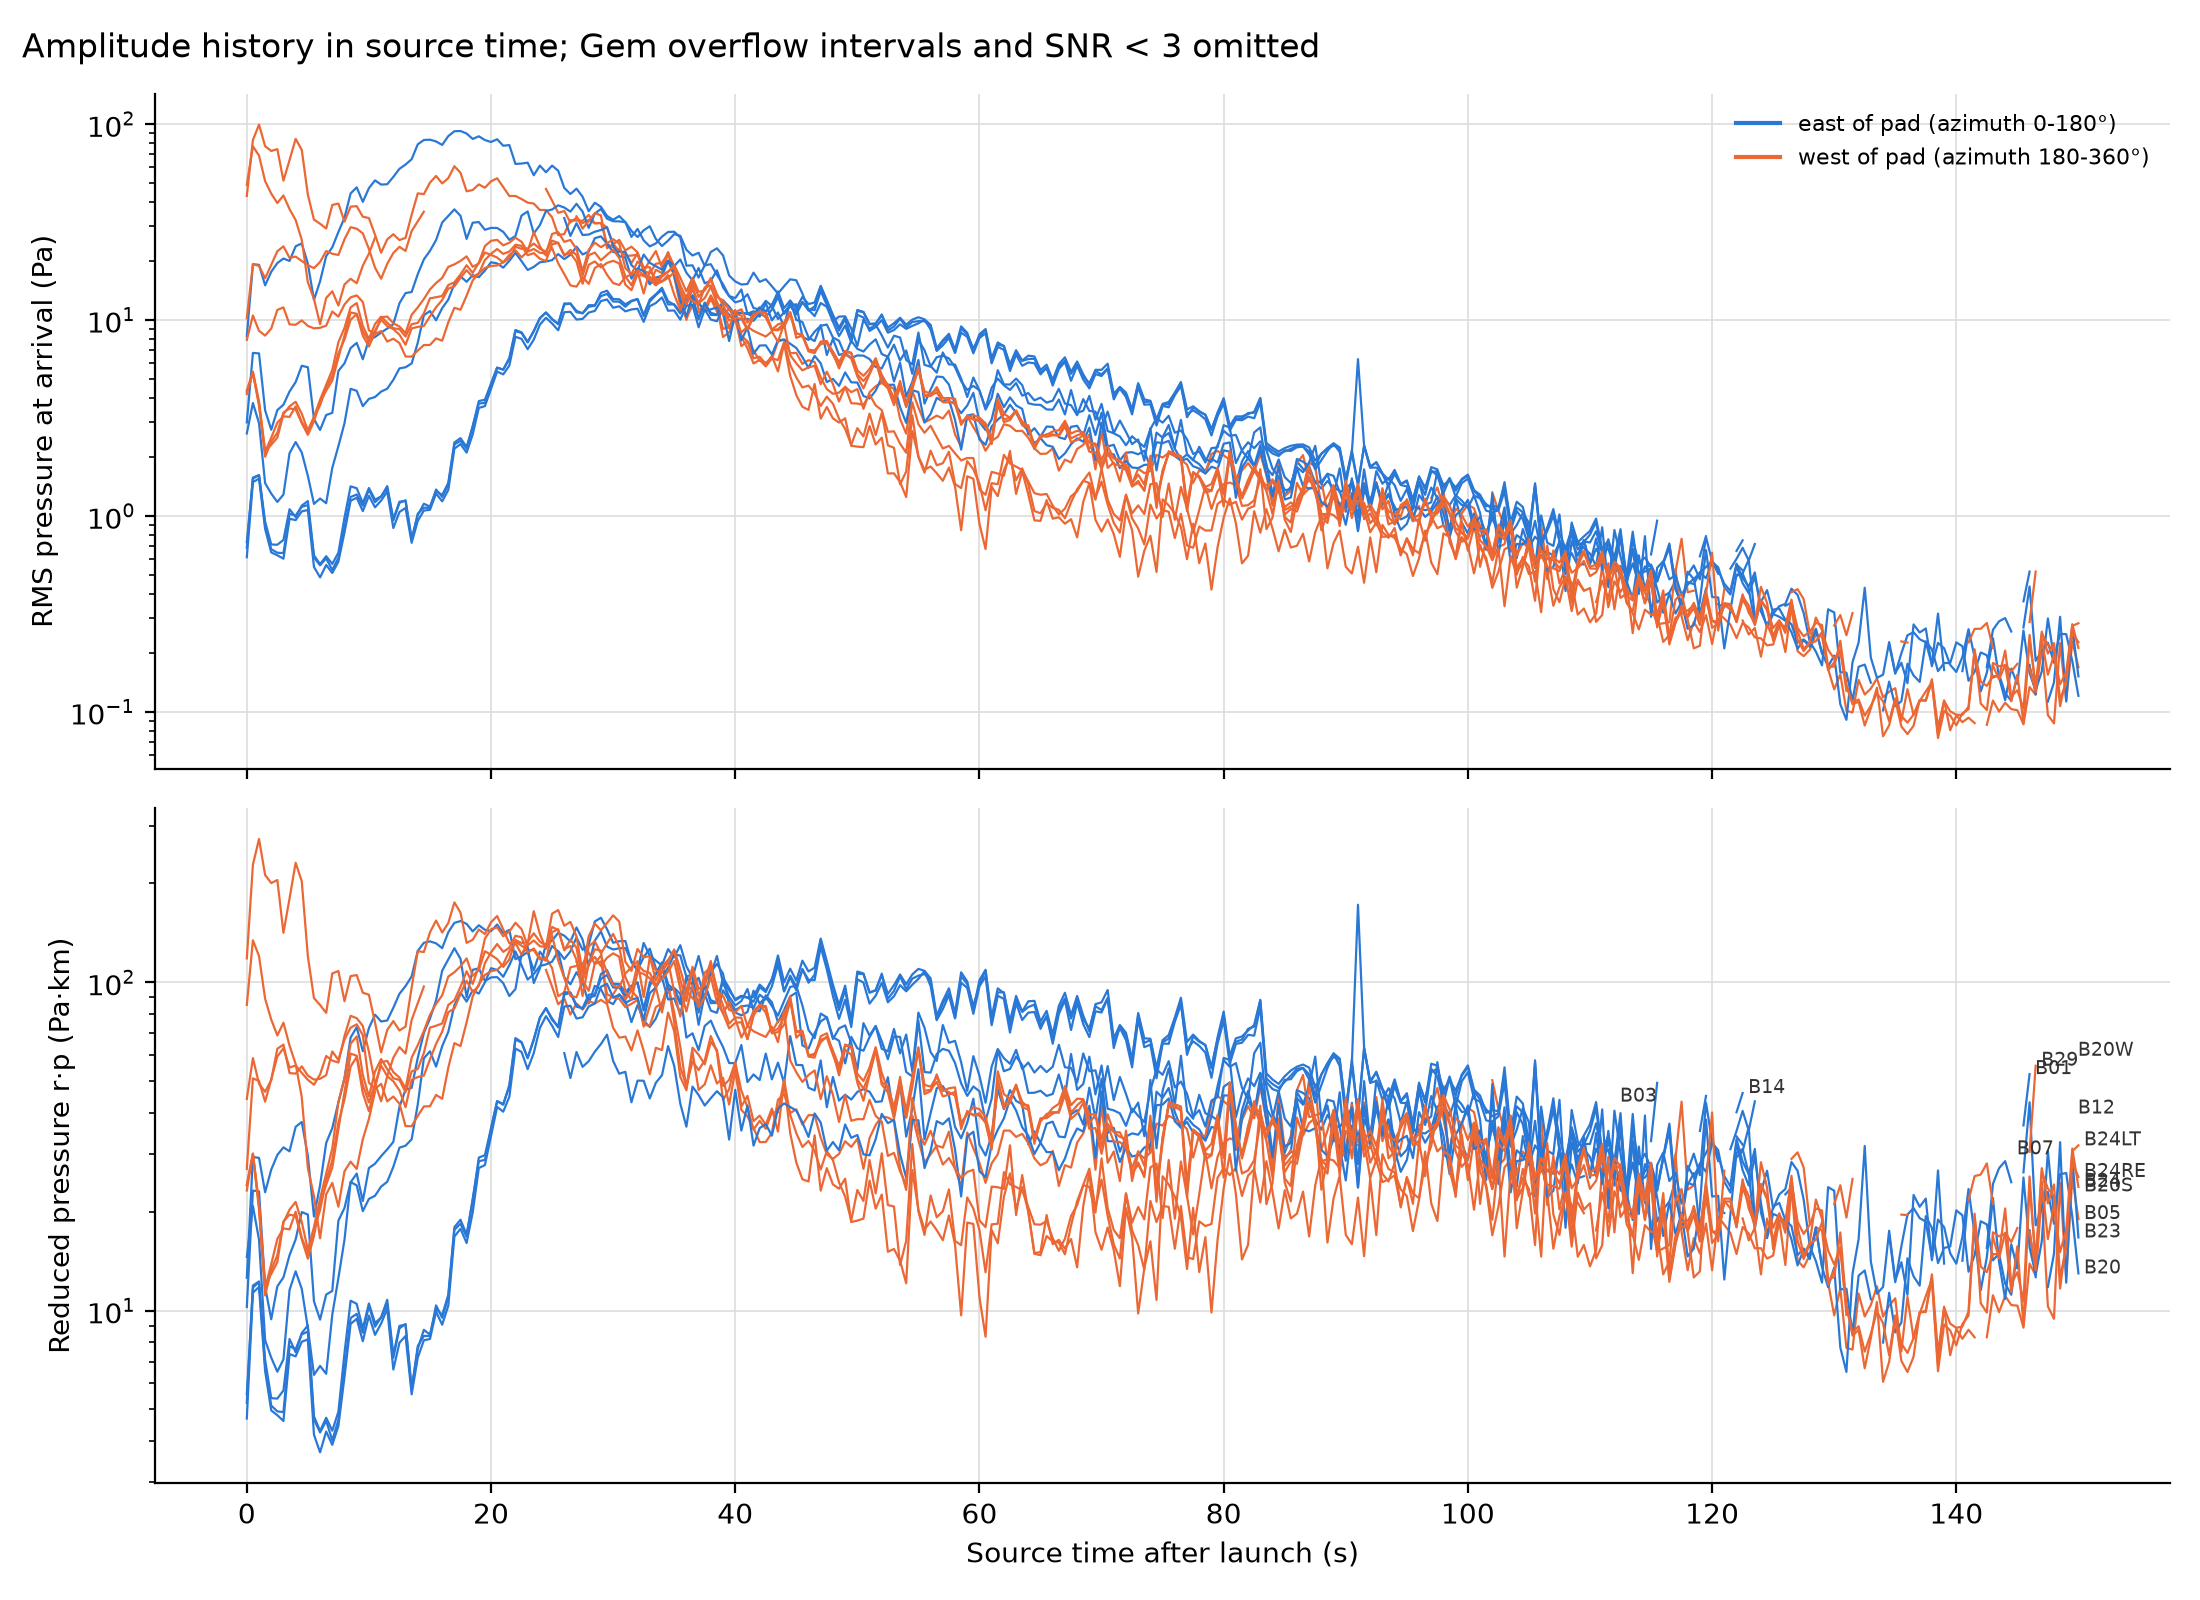
\includegraphics[width=\textwidth]{moving_source_reduced_pressure}
  \caption{Amplitude history in source time. Top: RMS pressure at the
    predicted arrival time for each source time. Bottom: reduced
    pressure $R(t_s)\,p$. Blue: stations east of the pad; orange:
    west. Gem overflow intervals and SNR~$<$~3 omitted.}
  \label{fig:reduced}
\end{figure}

\subsection{Empirical Directivity}

Plotting reduced pressure against the emission angle $\phi$ for all
stations and source times gives an empirical radiation pattern
(Figure~\ref{fig:model_data}a; \suppfig{1}). Reduced pressure is largest at
$\phi \approx 60$--70$^{\circ}$ from the exhaust axis and falls by a
factor of $\sim$5 towards $\phi \approx 10^{\circ}$; the binned
medians for source times 20--60~s and 60--150~s agree closely where
they overlap. Fitting a Gaussian cone (Equation~\ref{eq:directivity}) to the reduced
pressures for source times after the pad phase gives
$\phi_0 = 57^{\circ}$ and $\sigma = 26^{\circ}$ (source times
15--60~s; 58$^{\circ}$ and 29$^{\circ}$ for 15--120~s), with a scatter
of 0.12--0.13 log units. In this geometry, small
$\phi$ is reached only late in the flight, when the source is high and
far, so part of the decrease at small $\phi$ may reflect propagation
losses not in the model; the agreement between the two source-time
groups argues for a directivity effect.

%% ============================================================
\section{Forward Model with Data-Derived Directivity}
\label{sec:model}
\label{sec:modeling}
\label{sec:synthetics}

We represent the rocket as a point source on the trajectory of
Section~\ref{sec:trajectory}, with amplitude at a station
\begin{equation}
  A(t_s) \propto \frac{Q(t_s)\,D(\phi)}{R(t_s)},
  \label{eq:source}
\end{equation}
where $Q(t_s) = 1 - e^{-t_s/8\,\mathrm{s}}$ represents the build-up of
engine noise and $D(\phi)$ is a Gaussian cone,
\begin{equation}
  D(\phi) = \exp\!\left[-\frac{1}{2}\left(\frac{\phi - \phi_0}{\sigma}\right)^2\right].
  \label{eq:directivity}
\end{equation}
Our initial model assumed $\phi_0 = 30^{\circ}$ and $\sigma = 20^{\circ}$;
on idealized east and west station lines it predicts uprange stations
peaking earlier and 1.2--1.45 times louder than downrange stations, an
apparent speed of $\sim$125~m~s$^{-1}$ and amplitude decay as
$R^{-0.96}$ (\suppfig{2}, \suppfig{3}, \suppfig{4}). Here we instead use the
directivity measured in Section~\ref{sec:moving} ($\phi_0 = 57^{\circ}$,
$\sigma = 26^{\circ}$) and evaluate the model at the real station
positions. For each station we compare the time and amplitude of the
synthetic envelope peak with those of the observed RMS envelope (source
times $\geq$~10~s, overflow masked; amplitudes after one common scale
factor).

With the original cone, synthetic peaks arrive on average 21~s too late
(RMS error 25~s), because a 30$^{\circ}$ lobe sweeps across the stations
only once the vehicle is high and far. With the measured cone the RMS
error falls to 7~s with a mean bias of $-1$~s
(Figure~\ref{fig:model_data}), and the model's apparent speed (138~m~s$^{-1}$
for envelope peaks) approaches the observed value. Because the
directivity was fitted to amplitudes and not to times, this improvement
in timing is an independent test of the measured radiation pattern. The
relative amplitudes are matched equally well by both cones (0.20 log
units RMS); neither reproduces the full uprange/downrange contrast
(distance-corrected ratio 1.05 in the model versus 1.3 observed), nor the
pad phase, which the model does not include. The remaining misfit points
to the missing physics: the flame-trench source, an extended plume,
propagation through a real atmosphere, and the flown rather than the
nominal trajectory.

\begin{figure}[htbp]
  \centering
  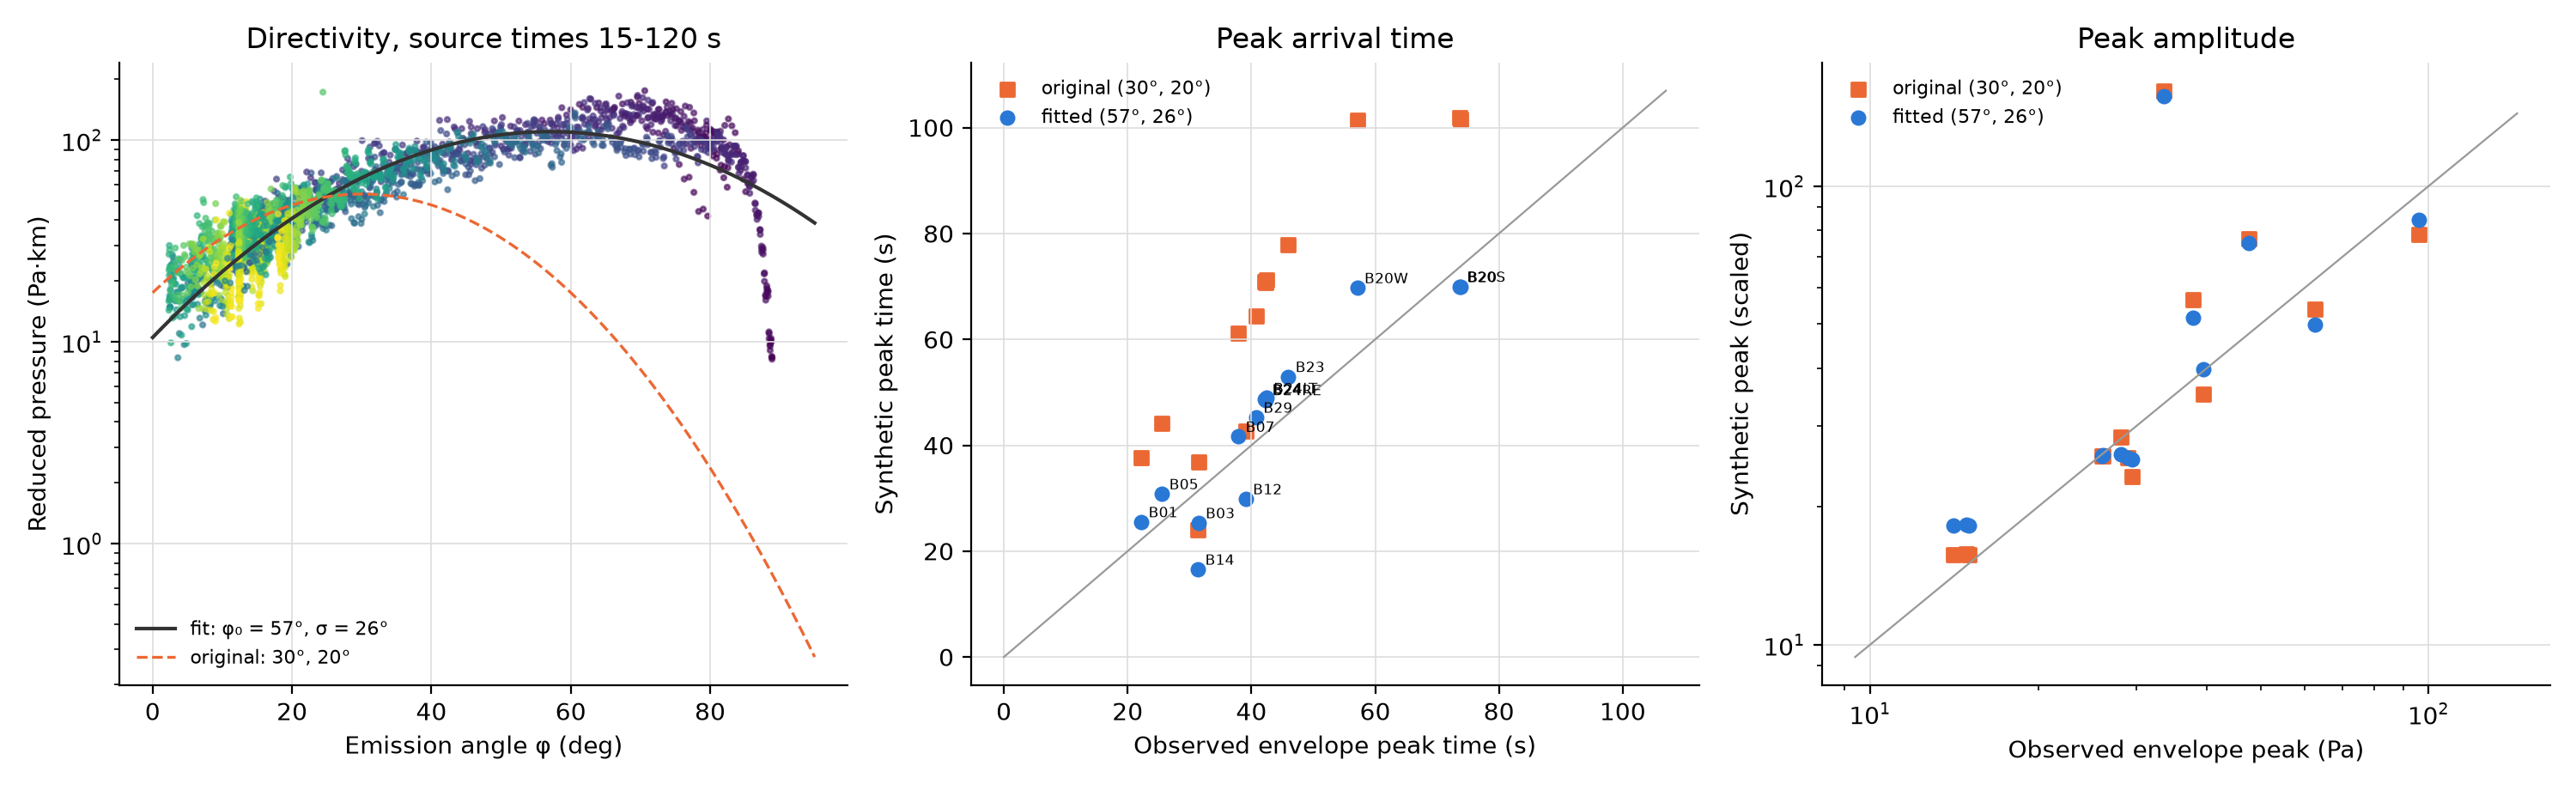
\includegraphics[width=\textwidth]{model_data_directivity}
  \caption{Left: reduced pressure against emission angle for source
    times 15--120~s, with the fitted Gaussian cone (black;
    $\phi_0 = 57^{\circ}$, $\sigma = 26^{\circ}$) and the originally
    assumed cone (orange dashed; 30$^{\circ}$, 20$^{\circ}$). Centre and
    right: synthetic versus observed envelope peak time and amplitude at
    each station for the two cones. The B14 observation is a lower bound
    (Gem overflow).}
  \label{fig:model_data}
\end{figure}


%% ============================================================
\section{Tracking the Vehicle with Small Infrasound Arrays}
\label{sec:arrays}

The B20 cluster (five Gems, aperture $\sim$35~m, element positions from
their own GPS logs, including Gem 363) and the B24 cluster (four Gems,
aperture $\sim$250~m) were analysed as arrays. In sliding windows (B20:
2~s, 2--10~Hz; B24: 4~s, 0.5--3~Hz), pairwise cross-correlation lags
were fitted with a plane wave to give the back-azimuth and trace
velocity, and the elevation angle $e$ from $\cos e = c/v_\text{trace}$.
Windows were accepted when the mean pairwise correlation exceeded 0.7;
median correlations were 0.98 (B20) and 0.95 (B24), with lag residuals
of 2.5 and 4.0~ms.

Both arrays track the vehicle from the first arrivals at $\sim$20~s to
180~s after launch (Figure~\ref{fig:arrays}a). Back-azimuths follow the
model for a launch azimuth of 90$^{\circ}$ throughout, including the
passage of the source to the north of B20 at $\sim$110~s. Elevation
angles agree with the model after $\sim$60~s, reaching 55--68$^{\circ}$;
before that the arrays measure $\sim$20$^{\circ}$ where the model predicts
near-grazing rays, a bias that could arise from near-surface wind or
temperature gradients changing the apparent sound speed, from sound
radiated by the extended plume above the vehicle, or from the small
aperture. Intersecting the two arrays' back-azimuths at common arrival
times locates the source in map view (Figure~\ref{fig:arrays}b): the
intersections begin within a few hundred metres of SLC-39B and follow a
track due east to $\sim$15~km downrange, within $\sim$0.5~km of the
model ground track. Two small arrays of low-cost sensors therefore
suffice to follow the ascent acoustically.

\begin{figure}[htbp]
  \centering
  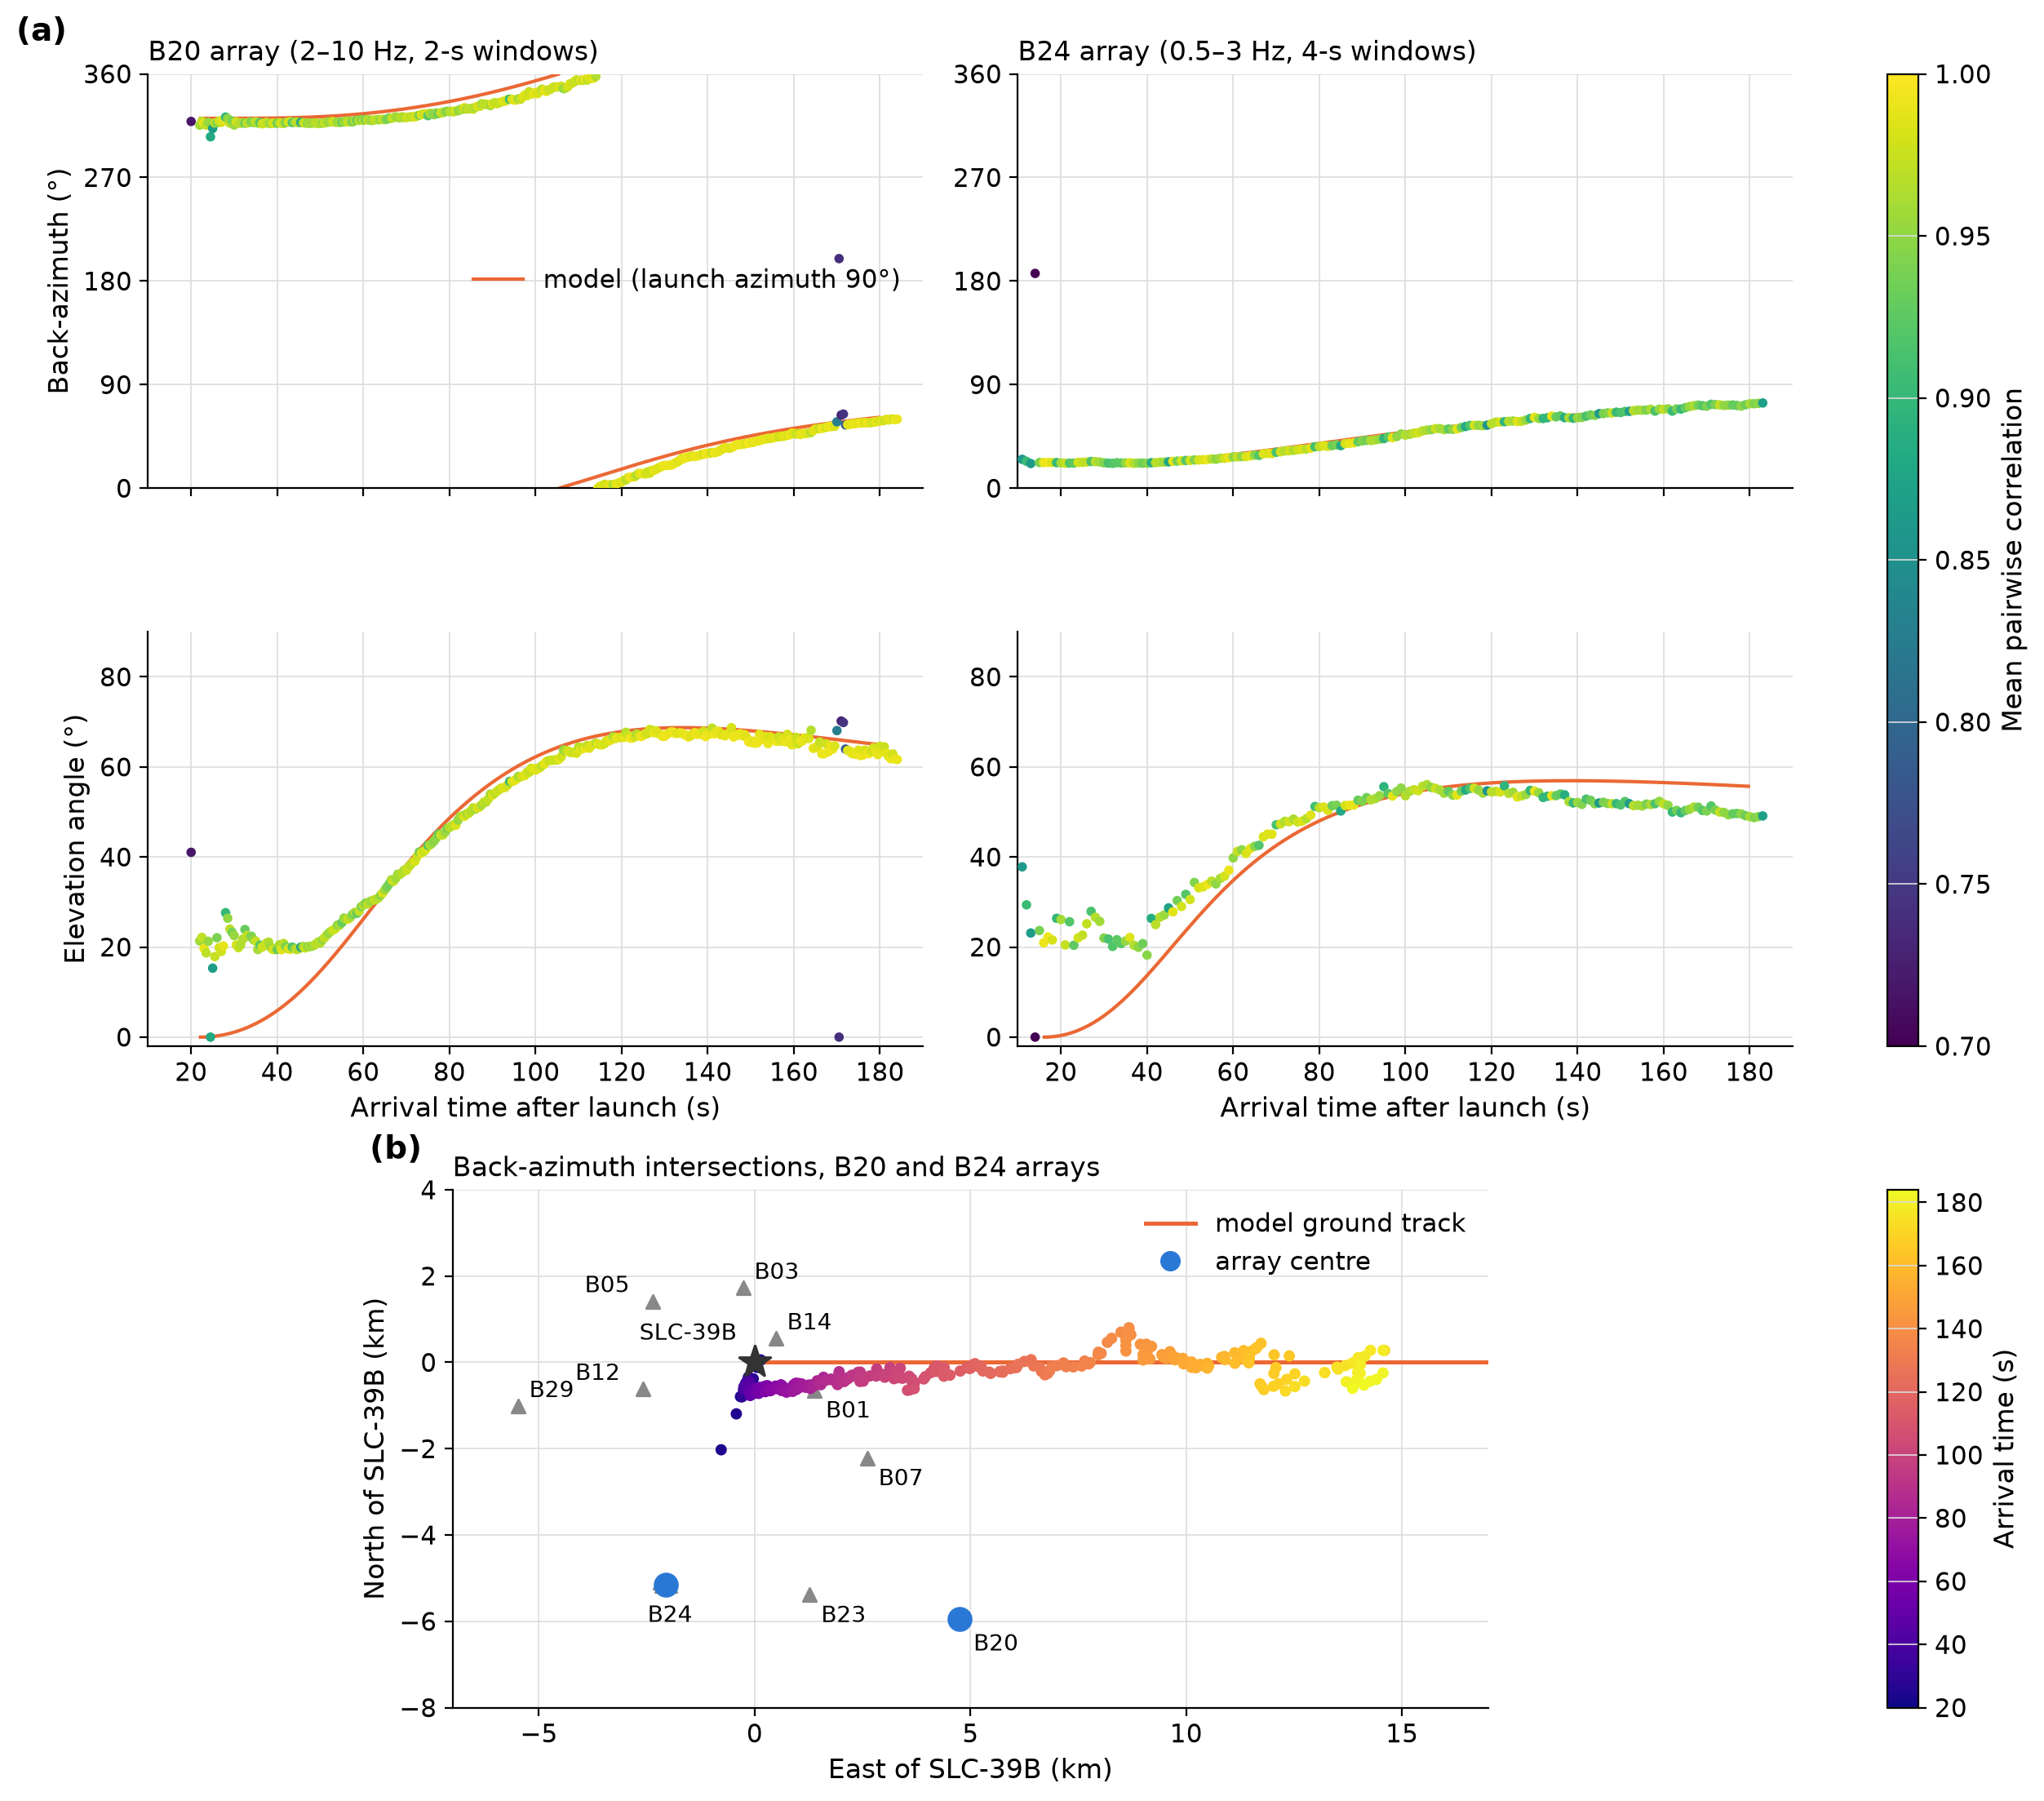
\includegraphics[width=\textwidth]{arrays_figure}
  \caption{(a) Back-azimuth (top) and elevation angle (bottom) from the B20
    (left) and B24 (right) arrays, coloured by mean pairwise correlation,
    against the straight-ray model for a launch azimuth of 90$^{\circ}$
    (orange). (b) Intersections of the two arrays' back-azimuths at common
    arrival times, coloured by arrival time, with the model ground track
    (orange) and the array centres (blue).}
  \label{fig:arrays}
\end{figure}

%% ============================================================
\section{Crackle}
\label{sec:crackle}

Crackle is the impulsive, popping component of jet and rocket noise
produced by steep shock fronts, which make the pressure waveform and
especially its time derivative positively skewed
\citep{FfowcsWilliams1975,Gee2013,McInerny1996}. Using the
500~samples~s$^{-1}$ infraBSUs at B01, B05 and B29 (high-passed at
1~Hz), we computed in 4-s windows the overall sound pressure level, the
skewness of pressure $Sk(p)$, the skewness of its time derivative
$Sk(\partial p/\partial t)$, and the rate of steep fronts (positive
derivative excursions above five times its RMS), and mapped each window
to its source time (Figure~\ref{fig:crackle}b). Windows within 15~dB of
the pre-launch noise level were discarded; in pre-launch noise both
skewnesses are $\sim$0.

Derivative skewness rises from $\sim$0 during the first 8~s at B01 and
B29 to 1.1--1.9 (median) for source times of 10--45~s, with maxima of
2.0--2.4, and declines afterwards (Figure~\ref{fig:crackle}b). Pressure
skewness reaches 0.3 (median) and exceeds the conventional crackle
threshold of $\sim$0.4 \citep{FfowcsWilliams1975} in many windows at
B01 in this interval. The crackle-producing interval corresponds to the
vehicle at $\sim$0.2--6~km altitude and subsonic (the model passes
Mach~1 only at $\sim$48~s), so the crackle arises in the supersonic
exhaust jet rather than from the vehicle's motion. At B05, the
first $\sim$9~s also exceed $Sk(p) = 0.4$, associated with the impulsive
ignition overpressure. Derivative skewness is larger at B29 (5.6~km;
median 1.9) than at B01 (1.5~km; 1.3) for the same source times, while
pressure skewness decreases with distance, consistent with nonlinear
steepening of the waveform during propagation \citep{Gee2008}; example
waveforms are shown in Figure~\ref{fig:crackle}a. This is the crackle heard by
observers: at 5.6~km it arrives 25--70~s after liftoff.

Derivative skewness depends strongly on sampling rate because the shock
rise is not resolved: after decimation to 100~samples~s$^{-1}$, median
$Sk(\partial p/\partial t)$ in the loudest minute falls to
$\sim$40\% of its 500~samples~s$^{-1}$ value, whereas $Sk(p)$ is less
affected. Crackle therefore cannot be quantified from the Gem
recordings. The infraBSUs were themselves housed in plastic totes that also
contained the station electronics; the totes' wall resonances alter the
spectrum above $\sim$10~Hz by up to $\sim$3~dB at 10--40~Hz at B29, and
their effect above 50~Hz, where the derivative skewness draws much of its
weight, could not be measured. The crackle metrics are therefore best
compared between these three stations, which share the same enclosure
design, rather than taken as absolute free-field values.

\begin{figure}[htbp]
  \centering
  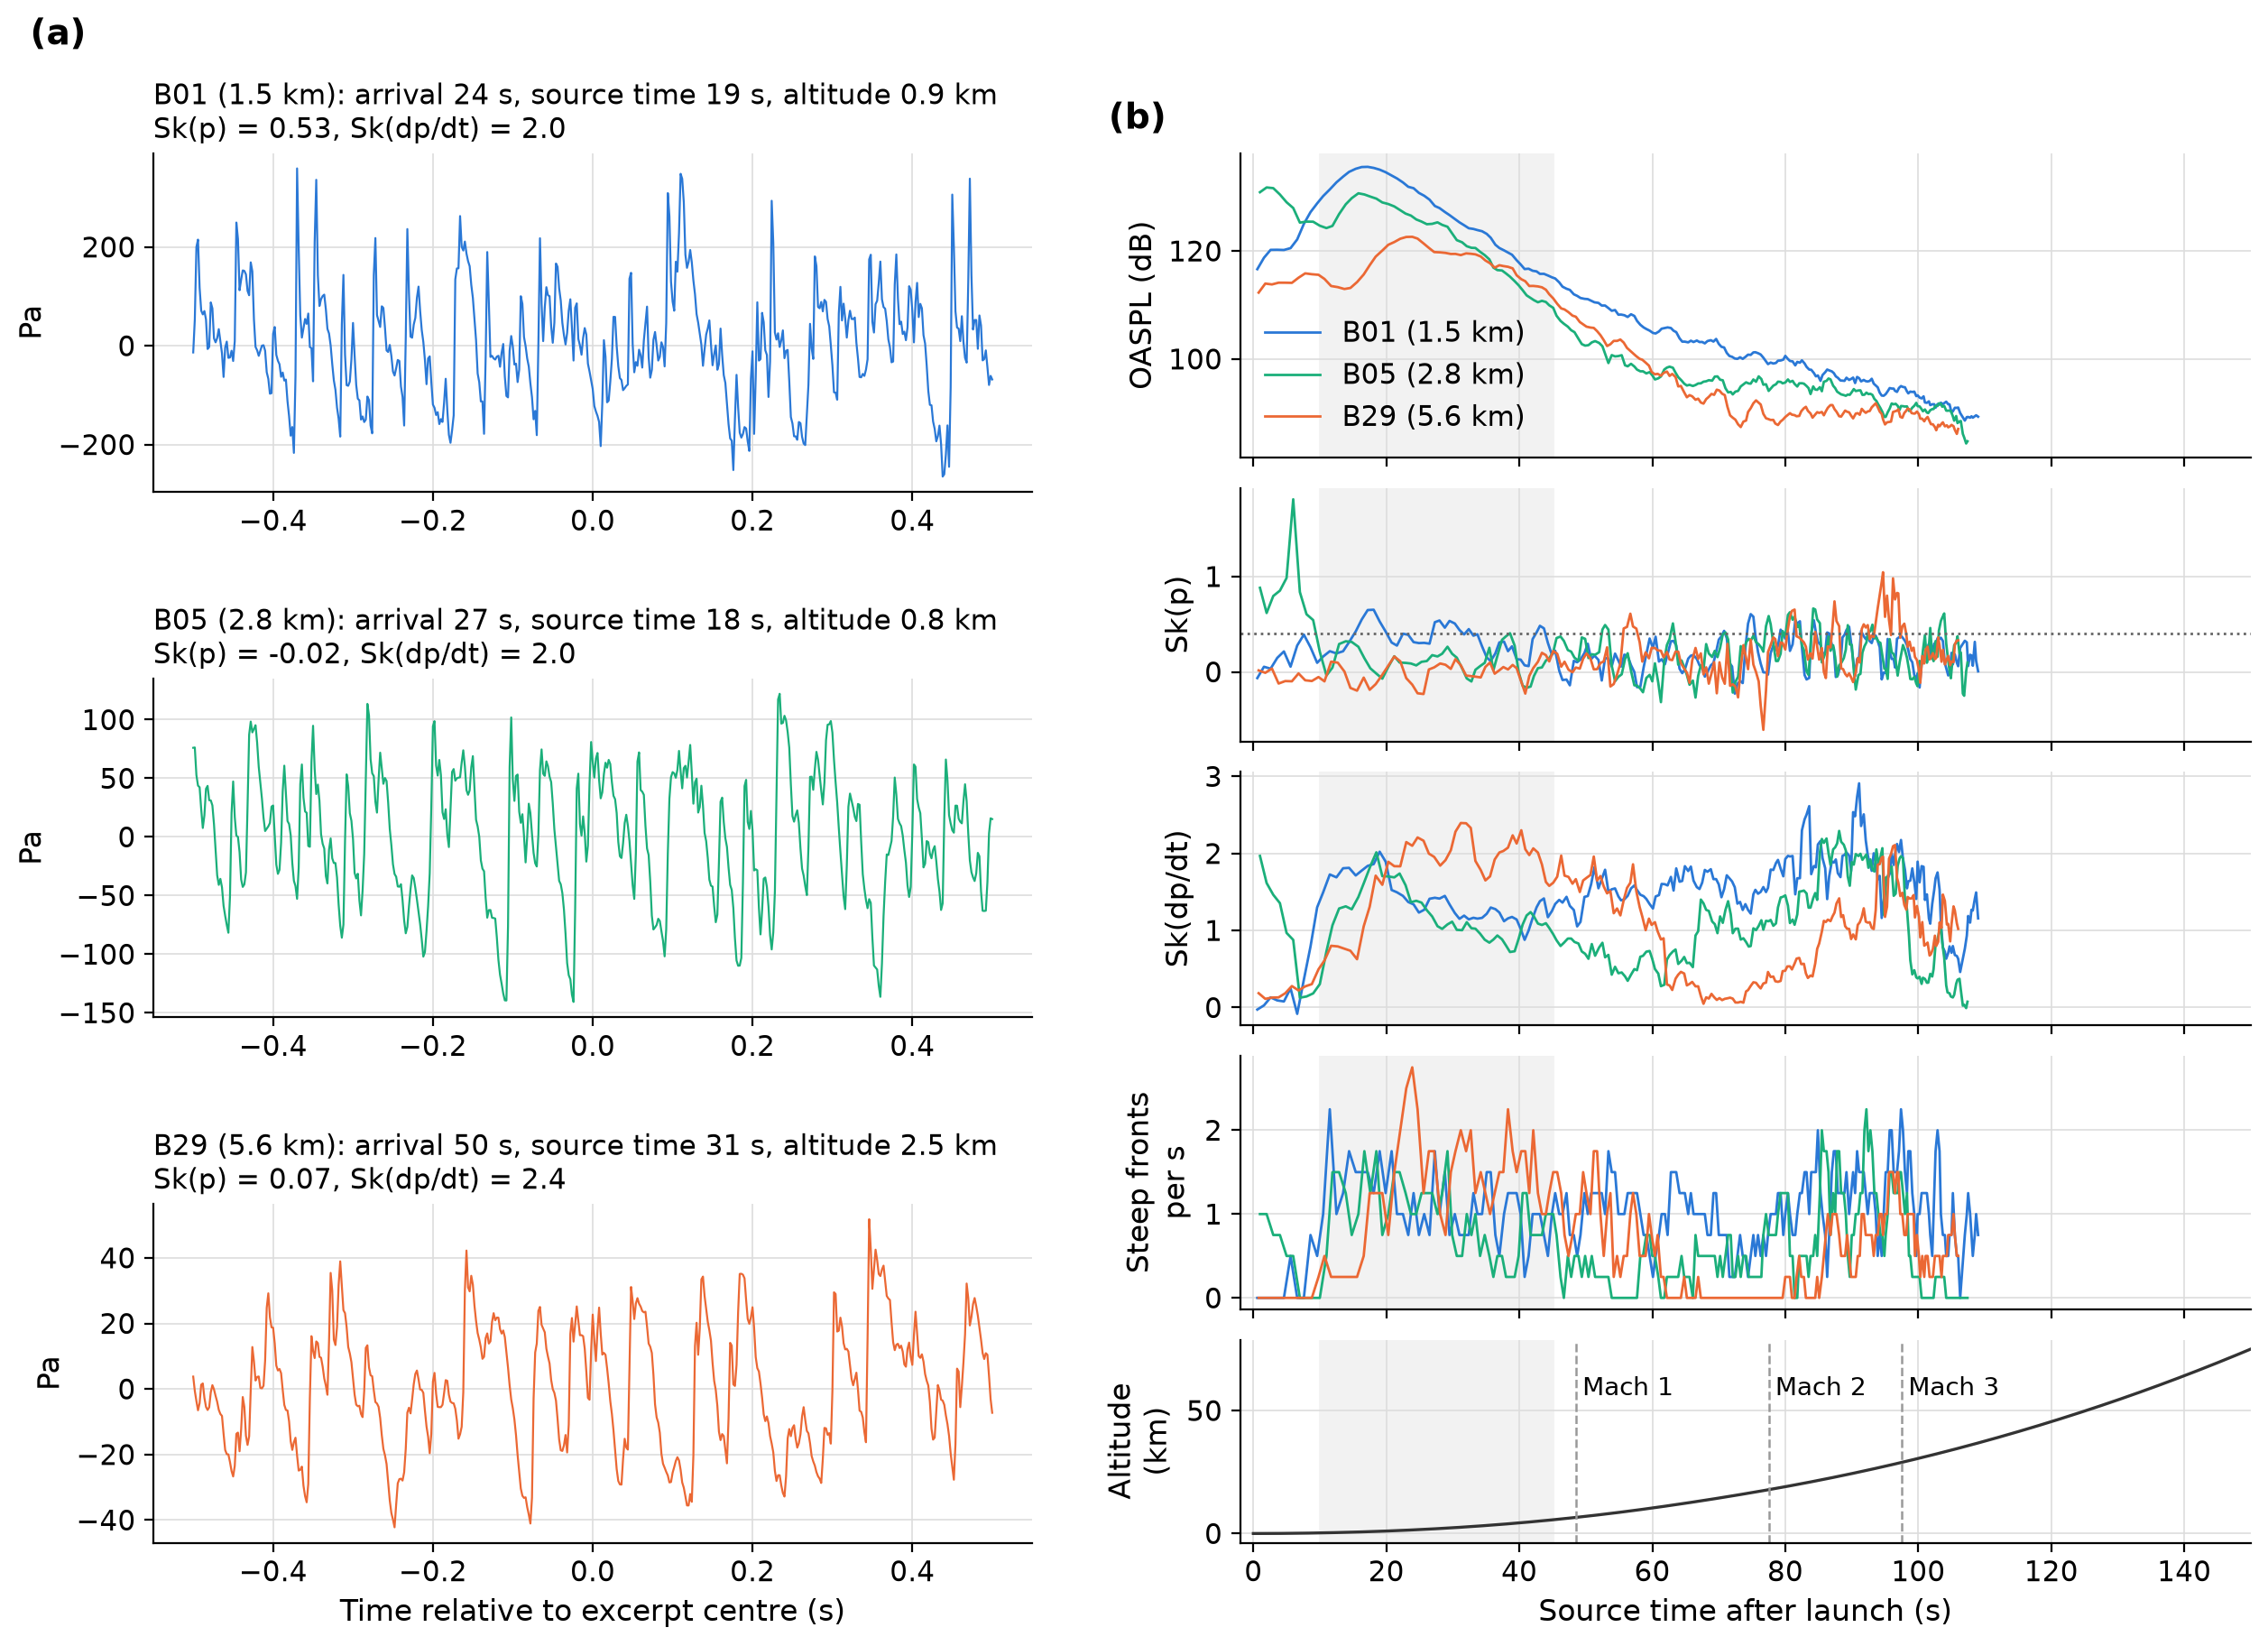
\includegraphics[width=\textwidth]{crackle_figure}
  \caption{(a) One-second excerpts with the largest derivative skewness at
    B01, B05 and B29 for source times 10--45~s, showing steep pressure rises
    followed by slower decays. (b) Crackle metrics in 4-s windows at the three
    infraBSU stations, plotted at the source time of emission: overall sound
    pressure level, pressure skewness (dotted: 0.4), derivative skewness,
    steep-front rate, and the model altitude with Mach-number crossings.
    Shaded: source times 10--45~s used for summary values.}
  \label{fig:crackle}
\end{figure}


%% ============================================================
\section{Discussion}

\subsection{What Controls the Infrasound Observations?}

Three factors dominate. First, the moving source: peak amplitudes and
arrival times at different distances sample different parts of the
trajectory, which produces the slow apparent speed (127~m~s$^{-1}$) and
contributes to the steep pressure decay ($r^{-1.40}$). Second,
directivity: the empirical pattern peaks at 60--70$^{\circ}$ from the
exhaust axis, uprange stations are $\sim$1.4 times louder at a given
distance in peak pressure, and downrange stations remain louder later in
the flight. Third, the pad: the earliest and, at northern stations, the
strongest radiation comes from ignition and the flame trench, before the
vehicle has moved. A point source on the vehicle with the measured
directivity cone (57$^{\circ}$) reproduces peak arrival times to
$\sim$7~s, much better than the 30$^{\circ}$ cone initially assumed,
but not the full azimuthal contrast or the pad phase.

\subsection{Limitations}

The forward model assumes a constant sound speed, straight rays, no
wind, a point source with a fixed directivity cone, and a nominal
trajectory rather than the flown one; the launch azimuth was supported
by the arrays but not fitted. Straight rays become increasingly
approximate after $\sim$60~s. The infraBSU response above $\sim$100~Hz is
nominal, and the infraBSUs were housed in electronics totes whose wall
resonances affect frequencies above $\sim$10~Hz (\paperone). The
farther stations are all 100~samples~s$^{-1}$ Gems, which underestimate
peak pressure and cannot resolve crackle.

\subsection{Implications}

Rocket launches are controlled geophysical sources with known origin
time and location. Source-time mapping turns a network of fixed stations
into a scan of the radiation pattern over a wide range of emission
angles, and small arrays of low-cost sensors add an independent check on
the source position. The same approach applies to other moving or
extended sources such as bolides and volcanic jets, and Artemis~II
provides a template for analysing the multi-year record of launches from
Kennedy Space Center. The infrasound yield-estimation approach applied to
accidental explosions \citep{silber_scamfer_newglenn_2026} and to
regional propagation of rocket signals \citep{Pilger2021} represents a
complementary use of networks such as this one.
\todo{Expand: relation to jet-noise directivity studies; relevance to
volcano infrasound.}


%% ============================================================
\section{Conclusions}

%% DRAFT
\begin{itemize}
  \item Peak pressure decays as $r^{-1.40}$ and peak ground velocity as
    $r^{-1.05}$; uprange stations are $\sim$1.4 times louder in peak
    pressure; peak arrival times give an apparent speed of
    127~m~s$^{-1}$.
  \item Mapped to emission time, ignition overpressure dominates to the
    north of the pad, and most stations record their strongest
    distance-corrected sound from source times of 17--30~s.
  \item Radiation peaks at $\sim$57$^{\circ}$ from the exhaust axis; a
    point-source model with this directivity predicts peak arrival times
    to $\sim$7~s (25~s with a 30$^{\circ}$ cone).
  \item Two small Gem arrays track the vehicle's bearing from $\sim$20 to
    180~s and locate its ground track due east of the pad.
  \item Crackle is emitted while the vehicle is at $\sim$0.2--6~km and
    subsonic, steepens with distance, and requires
    500~samples~s$^{-1}$ to quantify.
  \item High frequencies decline as the vehicle climbs, faster along
    longer paths.
\end{itemize}
\todo{Convert to prose.}


%% ============================================================
\section*{Data and Code Availability}

Waveform data will be archived through EarthScope upon publication.
Analysis code (notebooks 05--60 in \texttt{09\_artemis2\_paper}) is
available at
\url{https://github.com/gthompson/KSCRocketSeismology}; the version used will be archived with a DOI on acceptance.
The analysis builds on ObsPy \citep{Beyreuther2010,krischer_obspy_2015}
and FlovoPy \citep{flovopy_2026}.
Supplementary Figures S1--S5 and Tables S1--S2 are provided in a separate file.

\begin{acknowledgements}
The SmartSolo instruments were provided by the EarthScope Primary
Instrument Center (EPIC). Gem infrasound nodes were provided by Boise
State University. \todo{Complete acknowledgements: Katherine, Don?,
Robert, John?, others? NASA MSFC. Any grants to acknowledge?}
\end{acknowledgements}

\section*{Author Contributions}

\todo{Complete CRediT author contributions statement.}

%% ============================================================
%% Bibliography style is set by seismica.cls (abbrvnat_seismica_upcasetitle.bst)
\bibliography{artemis2}  %% references go in artemis2.bib

\end{document}
